
%(BEGIN_QUESTION)
% Copyright 2006, Tony R. Kuphaldt, released under the Creative Commons Attribution License (v 1.0)
% This means you may do almost anything with this work of mine, so long as you give me proper credit

Calculate values for the following calibration table, for a displacer-type level transmitter measuring liquid level interface (densities = 50 lb/ft$^{3}$ and 70 lb/ft$^{3}$), with a calibration tolerance of $\pm$ 1\%:

$$\includegraphics[width=15.5cm]{i00687x01.eps}$$

% No blank lines allowed between lines of an \halign structure!
% I use comments (%) instead, so that TeX doesn't choke.

$$\vbox{\offinterlineskip
\halign{\strut
\vrule \quad\hfil # \ \hfil & 
\vrule \quad\hfil # \ \hfil & 
\vrule \quad\hfil # \ \hfil & 
\vrule \quad\hfil # \ \hfil & 
\vrule \quad\hfil # \ \hfil & 
\vrule \quad\hfil # \ \hfil \vrule \cr
\noalign{\hrule}
%
% First row
Interface & Percent of & Buoyant & Output signal & Output signal & Output signal \cr
%
% Another row
level (in) & span (\%) & force (lbs) & ideal (PSI) & min. (PSI) & max. (PSI) \cr
%
\noalign{\hrule}
%
% Another row
  & 0 &  &  &  &  \cr
%
\noalign{\hrule}
%
% Another row
  & 10 &  &  &  &  \cr
%
\noalign{\hrule}
%
% Another row
  & 25 &  &  &  &  \cr
%
\noalign{\hrule}
%
% Another row
  & 50 &  &  &  &  \cr
%
\noalign{\hrule}
%
% Another row
  & 75 &  &  &  &  \cr
%
\noalign{\hrule}
%
% Another row
  & 90 &  &  &  &  \cr
%
\noalign{\hrule}
%
% Another row
  & 100 &  &  &  &  \cr
%
\noalign{\hrule}
} % End of \halign 
}$$ % End of \vbox

Assume the following displacer characteristics:

\begin{itemize}
\item{} Shape: {\it cylindrical}
\item{} Length = 11 inches
\item{} Diameter = 1.5 inches
\item{} Dry weight = 2.7 lbs
\end{itemize}

\vskip 10pt

Be sure to show all your mathematical work so that your instructor will be able to check the conceptual validity of your technique(s).  A good way to check to see if you're solving the problem correctly is to check that each and every one of your intermediate calculations (i.e. the results you get mid-way during the process to arrive at the final answer) has real physical meaning.  {\bf If you truly understand what you are doing, you will be able to identify the correct unit of measurement for every intermediate result and also be able to show where that number applies to the scenario at hand}.


\vskip 20pt \vbox{\hrule \hbox{\strut \vrule{} {\bf Suggestions for Socratic discussion} \vrule} \hrule}

\begin{itemize}
\item{} How will this level transmitter respond if the gas pressure inside this vessel were to increase?
\item{} How will this level transmitter respond if the gas pressure inside this vessel were to decrease?
\item{} How will this level transmitter respond if the total liquid level were to decrease below the top of the displacer?
\item{} Does it matter for the calibration of the instrument whether or not the displacer is solid or hollow?  For example, suppose a technician were to exchange a solid displacer for the original (hollow) displacer -- would he or she have to recalibrate the instrument?
\item{} Demonstrate how to {\it estimate} numerical answers for this problem without using a calculator.
\end{itemize}

\underbar{file i00687}
%(END_QUESTION)





%(BEGIN_ANSWER)

\noindent
{\bf Partial answer:}

% No blank lines allowed between lines of an \halign structure!
% I use comments (%) instead, so that TeX doesn't choke.

$$\vbox{\offinterlineskip
\halign{\strut
\vrule \quad\hfil # \ \hfil & 
\vrule \quad\hfil # \ \hfil & 
\vrule \quad\hfil # \ \hfil & 
\vrule \quad\hfil # \ \hfil & 
\vrule \quad\hfil # \ \hfil & 
\vrule \quad\hfil # \ \hfil \vrule \cr
\noalign{\hrule}
%
% First row
Interface & Percent of & Buoyant & Output signal & Output signal & Output signal \cr
%
% Another row
level (in) & span (\%) & force (lbs) & ideal (PSI) & min. (PSI) & max. (PSI) \cr
%
\noalign{\hrule}
%
% Another row
 & 0 & & 3 &  &  \cr
%
\noalign{\hrule}
%
% Another row
 & 10 &  &  & 4.08 &  \cr
%
\noalign{\hrule}
%
% Another row
2.75 & 25 &  &  &  &  \cr
%
\noalign{\hrule}
%
% Another row
 & 50 & 0.6750 &  &  &  \cr
%
\noalign{\hrule}
%
% Another row
 & 75 &  &  &  & 12.12 \cr
%
\noalign{\hrule}
%
% Another row
9.9 & 90 &  &  &  &  \cr
%
\noalign{\hrule}
%
% Another row
 & 100 & 0.7874 &  &  &  \cr
%
\noalign{\hrule}
} % End of \halign 
}$$ % End of \vbox

%(END_ANSWER)





%(BEGIN_NOTES)

Here are the two ``thought experiment'' scenarios pictured to arrive at the LRV and URV pressure values:

$$\includegraphics[width=15.5cm]{i00687x02.eps}$$

% No blank lines allowed between lines of an \halign structure!
% I use comments (%) instead, so that TeX doesn't choke.

$$\vbox{\offinterlineskip
\halign{\strut
\vrule \quad\hfil # \ \hfil & 
\vrule \quad\hfil # \ \hfil & 
\vrule \quad\hfil # \ \hfil & 
\vrule \quad\hfil # \ \hfil & 
\vrule \quad\hfil # \ \hfil & 
\vrule \quad\hfil # \ \hfil \vrule \cr
\noalign{\hrule}
%
% First row
Interface & Percent of & Buoyant & Output signal & Output signal & Output signal \cr
%
% Another row
level (in) & span (\%) & force (lbs) & ideal (PSI) & min. (PSI) & max. (PSI) \cr
%
\noalign{\hrule}
%
% Another row
0 & 0 & 0.5625 & 3 & 2.88 & 3.12 \cr
%
\noalign{\hrule}
%
% Another row
1.1 & 10 & 0.5850 & 4.2 & 4.08 & 4.32 \cr
%
\noalign{\hrule}
%
% Another row
2.75 & 25 & 0.6187 & 6 & 5.88 & 6.12 \cr
%
\noalign{\hrule}
%
% Another row
5.5 & 50 & 0.6750 & 9 & 8.88 & 9.12 \cr
%
\noalign{\hrule}
%
% Another row
8.25 & 75 & 0.7312 & 12 & 11.88 & 12.12 \cr
%
\noalign{\hrule}
%
% Another row
9.9 & 90 & 0.7649 & 13.8 & 13.68 & 13.92 \cr
%
\noalign{\hrule}
%
% Another row
11 & 100 & 0.7874 & 15 & 14.88 & 15.12 \cr
%
\noalign{\hrule}
} % End of \halign 
}$$ % End of \vbox

\vskip 10pt

The 318 PSI and 135 $^{o}$F vapor space parameters are extraneous information, included for the purpose of challenging students to identify whether or not information is relevant to solving a particular problem.


%INDEX% Measurement, interface level: displacer (buoyancy)

%(END_NOTES)


